% Options for packages loaded elsewhere
\PassOptionsToPackage{unicode}{hyperref}
\PassOptionsToPackage{hyphens}{url}
%
\documentclass[
]{article}
\usepackage{amsmath,amssymb}
\usepackage{lmodern}
\usepackage{ifxetex,ifluatex}
\ifnum 0\ifxetex 1\fi\ifluatex 1\fi=0 % if pdftex
  \usepackage[T1]{fontenc}
  \usepackage[utf8]{inputenc}
  \usepackage{textcomp} % provide euro and other symbols
\else % if luatex or xetex
  \usepackage{unicode-math}
  \defaultfontfeatures{Scale=MatchLowercase}
  \defaultfontfeatures[\rmfamily]{Ligatures=TeX,Scale=1}
\fi
% Use upquote if available, for straight quotes in verbatim environments
\IfFileExists{upquote.sty}{\usepackage{upquote}}{}
\IfFileExists{microtype.sty}{% use microtype if available
  \usepackage[]{microtype}
  \UseMicrotypeSet[protrusion]{basicmath} % disable protrusion for tt fonts
}{}
\makeatletter
\@ifundefined{KOMAClassName}{% if non-KOMA class
  \IfFileExists{parskip.sty}{%
    \usepackage{parskip}
  }{% else
    \setlength{\parindent}{0pt}
    \setlength{\parskip}{6pt plus 2pt minus 1pt}}
}{% if KOMA class
  \KOMAoptions{parskip=half}}
\makeatother
\usepackage{xcolor}
\IfFileExists{xurl.sty}{\usepackage{xurl}}{} % add URL line breaks if available
\IfFileExists{bookmark.sty}{\usepackage{bookmark}}{\usepackage{hyperref}}
\hypersetup{
  pdftitle={Visualizations for soil2},
  pdfauthor={Frankie Fan},
  hidelinks,
  pdfcreator={LaTeX via pandoc}}
\urlstyle{same} % disable monospaced font for URLs
\usepackage[margin=1in]{geometry}
\usepackage{color}
\usepackage{fancyvrb}
\newcommand{\VerbBar}{|}
\newcommand{\VERB}{\Verb[commandchars=\\\{\}]}
\DefineVerbatimEnvironment{Highlighting}{Verbatim}{commandchars=\\\{\}}
% Add ',fontsize=\small' for more characters per line
\usepackage{framed}
\definecolor{shadecolor}{RGB}{248,248,248}
\newenvironment{Shaded}{\begin{snugshade}}{\end{snugshade}}
\newcommand{\AlertTok}[1]{\textcolor[rgb]{0.94,0.16,0.16}{#1}}
\newcommand{\AnnotationTok}[1]{\textcolor[rgb]{0.56,0.35,0.01}{\textbf{\textit{#1}}}}
\newcommand{\AttributeTok}[1]{\textcolor[rgb]{0.77,0.63,0.00}{#1}}
\newcommand{\BaseNTok}[1]{\textcolor[rgb]{0.00,0.00,0.81}{#1}}
\newcommand{\BuiltInTok}[1]{#1}
\newcommand{\CharTok}[1]{\textcolor[rgb]{0.31,0.60,0.02}{#1}}
\newcommand{\CommentTok}[1]{\textcolor[rgb]{0.56,0.35,0.01}{\textit{#1}}}
\newcommand{\CommentVarTok}[1]{\textcolor[rgb]{0.56,0.35,0.01}{\textbf{\textit{#1}}}}
\newcommand{\ConstantTok}[1]{\textcolor[rgb]{0.00,0.00,0.00}{#1}}
\newcommand{\ControlFlowTok}[1]{\textcolor[rgb]{0.13,0.29,0.53}{\textbf{#1}}}
\newcommand{\DataTypeTok}[1]{\textcolor[rgb]{0.13,0.29,0.53}{#1}}
\newcommand{\DecValTok}[1]{\textcolor[rgb]{0.00,0.00,0.81}{#1}}
\newcommand{\DocumentationTok}[1]{\textcolor[rgb]{0.56,0.35,0.01}{\textbf{\textit{#1}}}}
\newcommand{\ErrorTok}[1]{\textcolor[rgb]{0.64,0.00,0.00}{\textbf{#1}}}
\newcommand{\ExtensionTok}[1]{#1}
\newcommand{\FloatTok}[1]{\textcolor[rgb]{0.00,0.00,0.81}{#1}}
\newcommand{\FunctionTok}[1]{\textcolor[rgb]{0.00,0.00,0.00}{#1}}
\newcommand{\ImportTok}[1]{#1}
\newcommand{\InformationTok}[1]{\textcolor[rgb]{0.56,0.35,0.01}{\textbf{\textit{#1}}}}
\newcommand{\KeywordTok}[1]{\textcolor[rgb]{0.13,0.29,0.53}{\textbf{#1}}}
\newcommand{\NormalTok}[1]{#1}
\newcommand{\OperatorTok}[1]{\textcolor[rgb]{0.81,0.36,0.00}{\textbf{#1}}}
\newcommand{\OtherTok}[1]{\textcolor[rgb]{0.56,0.35,0.01}{#1}}
\newcommand{\PreprocessorTok}[1]{\textcolor[rgb]{0.56,0.35,0.01}{\textit{#1}}}
\newcommand{\RegionMarkerTok}[1]{#1}
\newcommand{\SpecialCharTok}[1]{\textcolor[rgb]{0.00,0.00,0.00}{#1}}
\newcommand{\SpecialStringTok}[1]{\textcolor[rgb]{0.31,0.60,0.02}{#1}}
\newcommand{\StringTok}[1]{\textcolor[rgb]{0.31,0.60,0.02}{#1}}
\newcommand{\VariableTok}[1]{\textcolor[rgb]{0.00,0.00,0.00}{#1}}
\newcommand{\VerbatimStringTok}[1]{\textcolor[rgb]{0.31,0.60,0.02}{#1}}
\newcommand{\WarningTok}[1]{\textcolor[rgb]{0.56,0.35,0.01}{\textbf{\textit{#1}}}}
\usepackage{graphicx}
\makeatletter
\def\maxwidth{\ifdim\Gin@nat@width>\linewidth\linewidth\else\Gin@nat@width\fi}
\def\maxheight{\ifdim\Gin@nat@height>\textheight\textheight\else\Gin@nat@height\fi}
\makeatother
% Scale images if necessary, so that they will not overflow the page
% margins by default, and it is still possible to overwrite the defaults
% using explicit options in \includegraphics[width, height, ...]{}
\setkeys{Gin}{width=\maxwidth,height=\maxheight,keepaspectratio}
% Set default figure placement to htbp
\makeatletter
\def\fps@figure{htbp}
\makeatother
\setlength{\emergencystretch}{3em} % prevent overfull lines
\providecommand{\tightlist}{%
  \setlength{\itemsep}{0pt}\setlength{\parskip}{0pt}}
\setcounter{secnumdepth}{-\maxdimen} % remove section numbering
\ifluatex
  \usepackage{selnolig}  % disable illegal ligatures
\fi

\title{Visualizations for soil2}
\author{Frankie Fan}
\date{2022-06-27}

\begin{document}
\maketitle

\begin{Shaded}
\begin{Highlighting}[]
\FunctionTok{library}\NormalTok{(readxl)}
\FunctionTok{library}\NormalTok{(dplyr)}
\end{Highlighting}
\end{Shaded}

\begin{verbatim}
## Warning: package 'dplyr' was built under R version 4.1.3
\end{verbatim}

\begin{verbatim}
## 
## Attaching package: 'dplyr'
\end{verbatim}

\begin{verbatim}
## The following objects are masked from 'package:stats':
## 
##     filter, lag
\end{verbatim}

\begin{verbatim}
## The following objects are masked from 'package:base':
## 
##     intersect, setdiff, setequal, union
\end{verbatim}

\begin{Shaded}
\begin{Highlighting}[]
\FunctionTok{library}\NormalTok{(tidyverse)}
\end{Highlighting}
\end{Shaded}

\begin{verbatim}
## Warning: package 'tidyverse' was built under R version 4.1.3
\end{verbatim}

\begin{verbatim}
## -- Attaching packages --------------------------------------- tidyverse 1.3.1 --
\end{verbatim}

\begin{verbatim}
## v ggplot2 3.3.5     v purrr   0.3.4
## v tibble  3.1.5     v stringr 1.4.0
## v tidyr   1.1.4     v forcats 0.5.1
## v readr   2.0.2
\end{verbatim}

\begin{verbatim}
## -- Conflicts ------------------------------------------ tidyverse_conflicts() --
## x dplyr::filter() masks stats::filter()
## x dplyr::lag()    masks stats::lag()
\end{verbatim}

\begin{Shaded}
\begin{Highlighting}[]
\FunctionTok{library}\NormalTok{(sf)}
\end{Highlighting}
\end{Shaded}

\begin{verbatim}
## Warning: package 'sf' was built under R version 4.1.3
\end{verbatim}

\begin{verbatim}
## Linking to GEOS 3.9.1, GDAL 3.2.1, PROJ 7.2.1; sf_use_s2() is TRUE
\end{verbatim}

\begin{Shaded}
\begin{Highlighting}[]
\FunctionTok{library}\NormalTok{(ggplot2)}
\FunctionTok{library}\NormalTok{(rgdal)}
\end{Highlighting}
\end{Shaded}

\begin{verbatim}
## Warning: package 'rgdal' was built under R version 4.1.3
\end{verbatim}

\begin{verbatim}
## Loading required package: sp
\end{verbatim}

\begin{verbatim}
## Please note that rgdal will be retired by the end of 2023,
## plan transition to sf/stars/terra functions using GDAL and PROJ
## at your earliest convenience.
## 
## rgdal: version: 1.5-32, (SVN revision 1176)
## Geospatial Data Abstraction Library extensions to R successfully loaded
## Loaded GDAL runtime: GDAL 3.4.1, released 2021/12/27
## Path to GDAL shared files: C:/Users/Alion/Documents/R/win-library/4.1/rgdal/gdal
## GDAL binary built with GEOS: TRUE 
## Loaded PROJ runtime: Rel. 7.2.1, January 1st, 2021, [PJ_VERSION: 721]
## Path to PROJ shared files: C:/Users/Alion/Documents/R/win-library/4.1/rgdal/proj
## PROJ CDN enabled: FALSE
## Linking to sp version:1.4-7
## To mute warnings of possible GDAL/OSR exportToProj4() degradation,
## use options("rgdal_show_exportToProj4_warnings"="none") before loading sp or rgdal.
\end{verbatim}

\begin{Shaded}
\begin{Highlighting}[]
\FunctionTok{library}\NormalTok{(ggsn)}
\end{Highlighting}
\end{Shaded}

\begin{verbatim}
## Warning: package 'ggsn' was built under R version 4.1.3
\end{verbatim}

\begin{verbatim}
## Loading required package: grid
\end{verbatim}

\begin{Shaded}
\begin{Highlighting}[]
\FunctionTok{library}\NormalTok{(ggspatial)}
\end{Highlighting}
\end{Shaded}

\begin{verbatim}
## Warning: package 'ggspatial' was built under R version 4.1.3
\end{verbatim}

read in the files \#variables already loaded from
dataProcessing-Soil.rmd

\begin{Shaded}
\begin{Highlighting}[]
\NormalTok{soil\_monthly }\OtherTok{\textless{}{-}} \FunctionTok{read\_csv}\NormalTok{(}\StringTok{"./Data/soil\_monthly.csv"}\NormalTok{)}
\end{Highlighting}
\end{Shaded}

\begin{verbatim}
## Rows: 4800 Columns: 6
## -- Column specification --------------------------------------------------------
## Delimiter: ","
## chr (2): District, MonthBegin
## dbl (4): YearBegin, AverageSoilMoisture, MaxSoilMoisture, MinSoilMoisture
## 
## i Use `spec()` to retrieve the full column specification for this data.
## i Specify the column types or set `show_col_types = FALSE` to quiet this message.
\end{verbatim}

\begin{Shaded}
\begin{Highlighting}[]
\NormalTok{soil\_annual }\OtherTok{\textless{}{-}} \FunctionTok{read\_csv}\NormalTok{(}\StringTok{"./Data/soil\_annual.csv"}\NormalTok{)}
\end{Highlighting}
\end{Shaded}

\begin{verbatim}
## Rows: 420 Columns: 5
## -- Column specification --------------------------------------------------------
## Delimiter: ","
## chr (1): District
## dbl (4): YearBegin, AverageSoilMoisture, MaxSoilMoisture, MinSoilMoisture
## 
## i Use `spec()` to retrieve the full column specification for this data.
## i Specify the column types or set `show_col_types = FALSE` to quiet this message.
\end{verbatim}

\begin{Shaded}
\begin{Highlighting}[]
\NormalTok{zim\_district }\OtherTok{\textless{}{-}} \FunctionTok{st\_read}\NormalTok{(}\StringTok{"./shape60/gadm36\_ZWE\_2.shp"}\NormalTok{)  }
\end{Highlighting}
\end{Shaded}

\begin{verbatim}
## Reading layer `gadm36_ZWE_2' from data source 
##   `C:\Users\Alion\Documents\Ari\DSPG\zim\2022_DSPG_Zimbabwe\shape60\gadm36_ZWE_2.shp' 
##   using driver `ESRI Shapefile'
## Simple feature collection with 60 features and 13 fields
## Geometry type: POLYGON
## Dimension:     XY
## Bounding box:  xmin: 25.23703 ymin: -22.42028 xmax: 33.0563 ymax: -15.60884
## Geodetic CRS:  WGS 84
\end{verbatim}

\begin{Shaded}
\begin{Highlighting}[]
\NormalTok{soilDated }\OtherTok{\textless{}{-}} \FunctionTok{read\_csv}\NormalTok{(}\StringTok{"./Data/soilDated.csv"}\NormalTok{) }
\end{Highlighting}
\end{Shaded}

\begin{verbatim}
## Rows: 48720 Columns: 8
## -- Column specification --------------------------------------------------------
## Delimiter: ","
## chr (5): District, MonthBegin, DayBegin, MonthEnd, DayEnd
## dbl (3): YearBegin, YearEnd, SoilMoisture
## 
## i Use `spec()` to retrieve the full column specification for this data.
## i Specify the column types or set `show_col_types = FALSE` to quiet this message.
\end{verbatim}

Rename cols to match

\begin{Shaded}
\begin{Highlighting}[]
\NormalTok{zim\_district }\OtherTok{\textless{}{-}} \FunctionTok{rename}\NormalTok{(zim\_district, }\AttributeTok{District =}\NormalTok{ NAME\_2)}
\end{Highlighting}
\end{Shaded}

\begin{Shaded}
\begin{Highlighting}[]
\NormalTok{zim\_district }\OtherTok{\textless{}{-}}\NormalTok{ zim\_district }\SpecialCharTok{\%\textgreater{}\%} 
  \FunctionTok{select}\NormalTok{(District)}

\NormalTok{MonthlysoilbyDis }\OtherTok{\textless{}{-}}\FunctionTok{full\_join}\NormalTok{ (zim\_district, soil\_monthly, }\AttributeTok{by =} \StringTok{"District"}\NormalTok{)}
\end{Highlighting}
\end{Shaded}

\hypertarget{monthly-map-for-yearbegin-2011-and-2017}{%
\subsection{1. Monthly map for YearBegin 2011 and
2017}\label{monthly-map-for-yearbegin-2011-and-2017}}

\begin{Shaded}
\begin{Highlighting}[]
\CommentTok{\# Maximum soil by month}
\NormalTok{MaxMonthlysoil2017 }\OtherTok{\textless{}{-}}\NormalTok{ MonthlysoilbyDis }\SpecialCharTok{\%\textgreater{}\%} 
  \FunctionTok{filter}\NormalTok{(YearBegin }\SpecialCharTok{==} \DecValTok{2017}\NormalTok{) }\SpecialCharTok{\%\textgreater{}\%} 
  \FunctionTok{arrange}\NormalTok{(MonthBegin) }\SpecialCharTok{\%\textgreater{}\%} 
  \FunctionTok{ggplot}\NormalTok{() }\SpecialCharTok{+}
  \FunctionTok{geom\_sf}\NormalTok{(}\AttributeTok{size =} \DecValTok{1}\NormalTok{, }\AttributeTok{color =} \StringTok{"black"}\NormalTok{, }\FunctionTok{aes}\NormalTok{(}\AttributeTok{fill =}\NormalTok{ MaxSoilMoisture)) }\SpecialCharTok{+}
  \FunctionTok{coord\_sf}\NormalTok{() }\SpecialCharTok{+}
  \FunctionTok{scale\_fill\_viridis\_c}\NormalTok{(}\AttributeTok{option =} \StringTok{"G"}\NormalTok{, }\AttributeTok{direction =} \SpecialCharTok{{-}}\DecValTok{1}\NormalTok{) }\SpecialCharTok{+}
  \FunctionTok{facet\_wrap}\NormalTok{(}\SpecialCharTok{\textasciitilde{}}\NormalTok{MonthBegin) }\SpecialCharTok{+}
  \FunctionTok{ggtitle}\NormalTok{(}\StringTok{"Max soil in Zimbabwe {-} 2011"}\NormalTok{)}
\NormalTok{MaxMonthlysoil2017}
\end{Highlighting}
\end{Shaded}

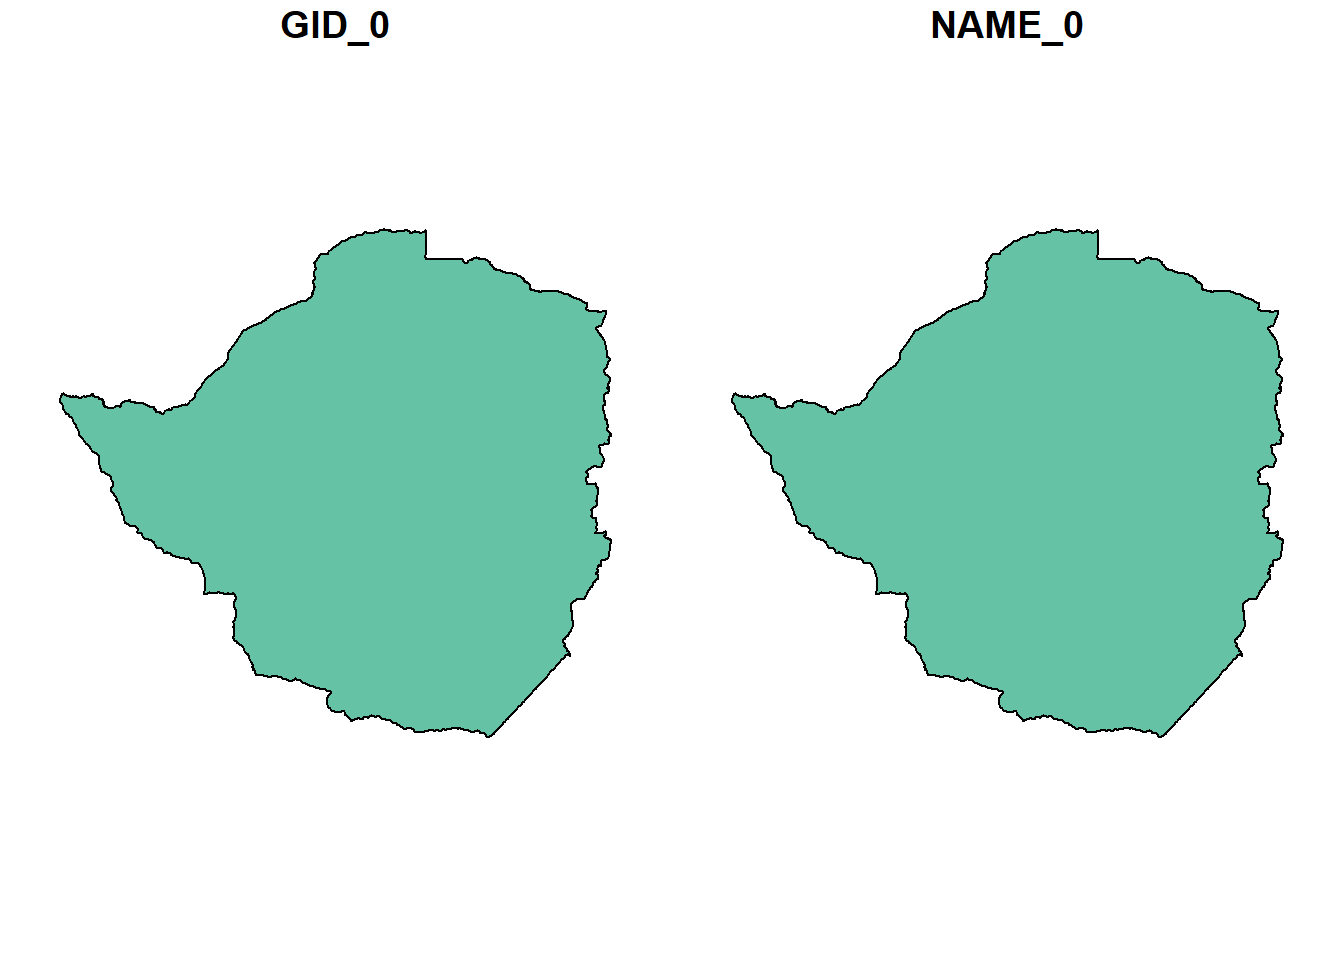
\includegraphics{Visualisations-for-soil2_files/figure-latex/unnamed-chunk-5-1.pdf}

\hypertarget{a.-distribution-of-soil-from-2011-2017}{%
\subsection{2a. Distribution of soil from
2011-2017}\label{a.-distribution-of-soil-from-2011-2017}}

\begin{Shaded}
\begin{Highlighting}[]
\NormalTok{soilDated }\SpecialCharTok{\%\textgreater{}\%} 
  \FunctionTok{filter}\NormalTok{( YearBegin }\SpecialCharTok{==} \DecValTok{2015}\SpecialCharTok{:} \DecValTok{2017}\NormalTok{) }\SpecialCharTok{\%\textgreater{}\%} 
  \FunctionTok{ggplot}\NormalTok{(}\FunctionTok{aes}\NormalTok{(}\AttributeTok{x =}\NormalTok{ YearBegin, }\AttributeTok{y =}\NormalTok{ SoilMoisture, }\AttributeTok{fill =} \FunctionTok{as.factor}\NormalTok{(YearBegin))) }\SpecialCharTok{+} 
  \FunctionTok{geom\_boxplot}\NormalTok{() }\SpecialCharTok{+}
  \FunctionTok{stat\_summary}\NormalTok{(}\AttributeTok{fun =} \StringTok{"mean"}\NormalTok{, }\AttributeTok{geom =} \StringTok{"point"}\NormalTok{, }\AttributeTok{shape =} \DecValTok{8}\NormalTok{,}
               \AttributeTok{size =} \DecValTok{2}\NormalTok{, }\AttributeTok{color =} \StringTok{"white"}\NormalTok{) }\SpecialCharTok{+}
  \FunctionTok{scale\_fill\_brewer}\NormalTok{(}\AttributeTok{palette=}\StringTok{"Set1"}\NormalTok{, }\AttributeTok{name =} \StringTok{"YearBegin"}\NormalTok{) }\SpecialCharTok{+}
  \FunctionTok{labs}\NormalTok{(}\AttributeTok{title =} \StringTok{"Distribution of soil in Zimbabwe, Year 2015 {-} 2017"}\NormalTok{) }
\end{Highlighting}
\end{Shaded}

\includegraphics{Visualisations-for-soil2_files/figure-latex/unnamed-chunk-6-1.pdf}

\hypertarget{b.-distribution-of-ndvi-in-2011-and-2017}{%
\subsection{2b. Distribution of NDVI in 2011 and
2017}\label{b.-distribution-of-ndvi-in-2011-and-2017}}

\begin{Shaded}
\begin{Highlighting}[]
\NormalTok{soil\_annual }\SpecialCharTok{\%\textgreater{}\%} 
  \FunctionTok{filter}\NormalTok{( YearBegin }\SpecialCharTok{==} \DecValTok{2015}\SpecialCharTok{|}\NormalTok{YearBegin }\SpecialCharTok{==} \DecValTok{2017}\NormalTok{) }\SpecialCharTok{\%\textgreater{}\%} 
  \FunctionTok{gather}\NormalTok{(Type, SoilMoisture, AverageSoilMoisture}\SpecialCharTok{:}\NormalTok{MinSoilMoisture) }\SpecialCharTok{\%\textgreater{}\%} 
  \FunctionTok{ggplot}\NormalTok{(}\FunctionTok{aes}\NormalTok{(}\AttributeTok{x =}\NormalTok{ Type, }\AttributeTok{y =}\NormalTok{ SoilMoisture, }\AttributeTok{fill =}\NormalTok{ Type)) }\SpecialCharTok{+}
  \FunctionTok{scale\_fill\_brewer}\NormalTok{(}\AttributeTok{palette=}\StringTok{"Set3"}\NormalTok{, }\AttributeTok{name =} \StringTok{"Type"}\NormalTok{) }\SpecialCharTok{+}
  \FunctionTok{facet\_wrap}\NormalTok{(}\SpecialCharTok{\textasciitilde{}}\NormalTok{YearBegin)}\SpecialCharTok{+}
  \FunctionTok{geom\_boxplot}\NormalTok{() }\SpecialCharTok{+}
  \FunctionTok{labs}\NormalTok{(}\AttributeTok{title =} \StringTok{"Distribution of soil, Year 2011 \& 2017"}\NormalTok{) }\SpecialCharTok{+}
    \FunctionTok{xlab}\NormalTok{(}\StringTok{"Statistics"}\NormalTok{) }\SpecialCharTok{+}
    \FunctionTok{ylab}\NormalTok{(}\StringTok{"soil"}\NormalTok{)}
\end{Highlighting}
\end{Shaded}

\includegraphics{Visualisations-for-soil2_files/figure-latex/unnamed-chunk-7-1.pdf}

\hypertarget{map-for-soil-in-march-in-2011-and-2017}{%
\subsection{3. map for soil in March in 2011 and
2017}\label{map-for-soil-in-march-in-2011-and-2017}}

\begin{Shaded}
\begin{Highlighting}[]
\NormalTok{MaxMarch }\OtherTok{\textless{}{-}}\NormalTok{ MonthlysoilbyDis }\SpecialCharTok{\%\textgreater{}\%} 
  \FunctionTok{filter}\NormalTok{(YearBegin }\SpecialCharTok{==} \DecValTok{2016}\SpecialCharTok{|}\NormalTok{YearBegin }\SpecialCharTok{==} \DecValTok{2017}\NormalTok{, MonthBegin }\SpecialCharTok{==} \StringTok{"03"}\NormalTok{) }\SpecialCharTok{\%\textgreater{}\%} 
  \FunctionTok{ggplot}\NormalTok{() }\SpecialCharTok{+}
  \FunctionTok{geom\_sf}\NormalTok{(}\AttributeTok{size =} \DecValTok{1}\NormalTok{, }\AttributeTok{color =} \StringTok{"black"}\NormalTok{, }\FunctionTok{aes}\NormalTok{(}\AttributeTok{fill =}\NormalTok{ MaxSoilMoisture)) }\SpecialCharTok{+}
  \FunctionTok{facet\_wrap}\NormalTok{(}\SpecialCharTok{\textasciitilde{}}\NormalTok{YearBegin) }\SpecialCharTok{+}
  \FunctionTok{coord\_sf}\NormalTok{() }\SpecialCharTok{+}
  \FunctionTok{scale\_fill\_viridis\_c}\NormalTok{(}\AttributeTok{option =} \StringTok{"G"}\NormalTok{, }\AttributeTok{direction =} \SpecialCharTok{{-}}\DecValTok{1}\NormalTok{) }\SpecialCharTok{+}
  \FunctionTok{ggtitle}\NormalTok{(}\StringTok{"Maximum soil moisture in Zimbabwe {-} March"}\NormalTok{)}
\NormalTok{MaxMarch}
\end{Highlighting}
\end{Shaded}

\includegraphics{Visualisations-for-soil2_files/figure-latex/visualization for March-1.pdf}

\end{document}
